%\documentclass{sig-alternate-10pt}
\documentclass[10pt, conference, onecolumn]{IEEEtran}
% used for pseudocode
\usepackage{algorithm}
\usepackage{algpseudocode}
\usepackage{longtable}
\usepackage{color}
\usepackage{hyperref}
\usepackage{subfig}
\usepackage{graphics}
\usepackage{graphicx}
\usepackage[T1]{fontenc} % optional
\usepackage{amsmath}
\usepackage[cmintegrals]{newtxmath}
\usepackage{bm} % optional
\usepackage{microtype}
\usepackage{cleveref}
\usepackage{fancyvrb}

\begin{document}
%
% --- Author Metadata here ---
%\conferenceinfo{MobiCom}{'15 Paris, France}
%\CopyrightYear{2015} % Allows default copyright year (20XX) to be over-ridden - IF NEED BE.
%\crdata{0-12345-67-8/90/01}  % Allows default copyright data (0-89791-88-6/97/05) to be over-ridden - IF NEED BE.
% --- End of Author Metadata ---
\title{A Common Data Model for Tagged Event Streams: Version 13}
\maketitle

%\begin{table}[h]
%\caption{History}
%\begin{center}

\begin{longtable}{|c|p{17cm}|}
\hline
Version & Changes \\\hline
0.3 & \small
      added File and Flow subclasses to Object \newline  
	added Value object \newline
	added source to all entities \newline
	marked that tags discussion is still in progress \newline
	added location/size to the affects relation from obj to event
\\\hline
0.4 & \small 
	    revamp of the Events section \S~\ref{sec:conceptual:events} \newline
          revamp of the Objects section \S~\ref{sec:objects} \newline
          revamp of the Tags section \S~\ref{sec:tags} \newline
          updated Figure~\ref{fig:erd} mainly Tags and rename Flow to NetFlow
          incorporated material from tags writeup by Sekar/Venkat \newline
          placeholder for tag structure pending discussion with Venkat          
\\\hline
0.5 & \small 
        added description of some key attributes \newline
        added schema section \S~\ref{sec:syntax} showing typed schema \newline
        added memory subclass, disambiguate Value as its own entity \newline 
        moved location and size as optional attributes of event \newline
        made sequence an attribute of event \newline
        udpated provenance tag description (structure is work in progress)
\\\hline
0.6 &  \small
  Added SensorObject and SensorTypes to accommodate Android  \newline
  Renamed Source to InstrumentationSource and defined a set of them  \newline
  Added program point to event, and added blind event type  \newline
  Added principal, does not yet model authentication  \newline
  Added unique ids (uids) to all entities, important for streaming efficiency and for modeling edges  \newline
  Refactored Tags, now ProvenanceTag entity has tagExpression, and conf/integ tags as attributes  \newline
  Refactored timestamps, now long (we will add logical types when that is supported in IDL)  \newline
  Refactored Object inheritance for AbstractObject, File, Netflow, Memory, Sensor  \newline
  Added optional key-value pairs to all entities and edges for extensibility  \newline
  Added start and end timestamps to subject and unitid to model unit instrumentation \newline
  Specified optional vs mandatory fields \newline
  Added meta event concept using hasParent edge for event
  cleaned up  \S~\ref{sec:syntax}, included ref to the git repo which has the full schema definition and updated Fig. 1
\\\hline
0.7 &  \small
  Refactored Value; it is not a first class entity anymore, we made it an attribute of the event  \newline
  Tag expression modeled as a tree using ProvenanceTagNode  \newline
  Removed all edges previously associated with Value  \newline
  Refactored tags representation: added ProvenanceTagNode that uses tree representation  \newline
  Associated values with tags allowing run length encoding  \newline
  Added SOURCE\_WINDOWS\_DIFT\_FAROS to instrumentation sources  \newline
  Added attributes to Subject for env vars: imported/exported libs, process information  \newline
  Renamed SensorObject to SourceObject, representing generic source (sensor or other)  \newline
  Made subject pid, ppid mandatory 
\\\hline
0.8 & \small
 rename entity uid attribute back to uuid to avoid confusion with user id \newline
 rename SourceObject to SrcSinkObject: every sink can be a source but the opposite is not true \newline
 rename SourceType to SrcSinkType \newline
 add SourceType.SOURCE\_SINK\_IPC, MIT/ClearScope is using this to represent net flow and internal IPC \newline
 add SourceType.SOURCE\_SYSTEM\_PROPERTY for representing program property variables \newline
 added SOURCE\_FREEBSD\_DTRACE\_CADETS, SOURCE\_FREEBSD\_TESLA\_CADETS for CADETS system instrumentation sources \newline
 add EDGE\_FILE\_AFFECTS\_EVENT, EDGE\_NETFLOW\_AFFECT\_EVENT, EDGE\_MEMORY\_AFFECTS\_EVENT, \newline
 remove ProvenanceTagNode.numChildren, gets confusing with tag nodes referencing tagIds \newline
 add ProvenanceTagNode attribute tag to the objects which subsumes Integrity and Confidentiality tags and is more expressive \newline 
 add optional k/v pairs to the ProvenanceTagNode for flexibility, using this in ClearScope for program point keys \newline
 updated ProvenanceTagNode.value union, replaced string with long. This is to reference uuid for source/sink object \newline
 add SOURCE\_AUDIO to the SrcSinkTypes \newline
 add optional attribute Event.name, common across datasets \newline
 added unknown even types EVENT\_KERNEL\_UNKNOWN, EVENT\_APP\_UNKNOWN etc which will be used sparingly \newline
 added edge types EDGE\_EVENT\_AFFECTS\_SRCSINK, EDGE\_SRCSINK\_AFFECTS\_EVENT for generic source/sink objects \newline
 added Value.valueDataType to describe the type of the Event.parameters's value (not always byte[]) \newline 
 updated Value.tag run length encoding \newline
 added Event.threadId since adding a separate thread entity seems overkill when its not adding any info  
\\\hline
0.9 & \small
  added InstrumentationSource SOURCE\_LINUX\_BEEP\_TRACE \newline
  added EventType EVENT\_CLONE, EVENT\_RENAME, EVENT\_UNIT, EVENT\_UPDATE \newline
 added boolean isPipe field to FileObject \newline
  added 256 bit UUID for all entities instead of the long (long term solution) \newline
  added default value 0 for Event.sequence and made Event.timestampMicros optional, needed for synthetic events
   where time or order is not known (e.g. some TRACE events) \newline
  made MemoryObject.pageNumber optional \newline
  fix typo in SrcSinkType.SOURCE\_HEART\_RATE 
\\\hline
10 & \small
  add SubjectType.BASIC\_BLOCK \newline
  make Subject.startTimeMicros optional (for processes that have started before monitoring starts) \newline
  add ValueType enum and Value.type to distinguish input vs return values \newline
  make Value more expressive to allow complex data types i.e. add Value.components=array<Value> \newline
  add event types EVENT\_RECVFROM, EVENT\_RECVMSG \newline
  add InstrumentationSource.SOURCE\_LINUX\_THEIA \newline
  Create a new entity TagEntity with a uuid and a ProvenanceTagNode (and perhaps a InstrumentationSource)
   that we can use for Subjects and Objects and Events \newline
  add the EdgeTypes for subject/object/event tags and add an edge between events \newline
  EDGE\_EVENT\_CAUSED\_EVENT, EDGE\_FILE\_HAS\_TAG, EDGE\_NETFLOW\_HAS\_TAG, EDGE\_MEMORY\_HAS\_TAG, 
  EDGE\_SRCSINK\_HAS\_TAG, EDGE\_SUBJECT\_HAS\_TAG, EDGE\_EVENT\_HAS\_TAG \newline
  remove the AbstractObject.tag (replaced with the TagEntity and hasTag edge)
\\\hline
11 & \small
   added enum ValueDataType for typing primitive values and complex values \newline
   updated Value.valueDataType to be of type ValueDataType for stronger typing \newline
   Value.valueBytes should assume UTF\_32BE encoding for all characters and strings \newline
   updated docs for Value.tag, Value.size, and Value.valueBytes with examples \newline
   added TCCDMDatum.CDMVersion=11 field to keep the CDM version explicit in the data
\\\hline
12 & \small
  add VALUE\_DATA\_TYPE\_BOOL data type: a boolean will be represented as a single byte TRUE=1, FALSE=0 \newline
  Value.valueDataType is now mandatory, used to be optional \newline
  added flag Value.isNull = true for null values \newline
  added Value.runtimeDataType which is a string representing the runtime data type of the value \newline
  updated documentation for Value record
\\\hline
13 & \small
  add event types: EVENT\_SENDTO send through socket, EVENT\_SENDMSG send through socket, EVENT\_SHM share memory between processes \newline
  Add timestamp to TagEntity since multiple tags may be associated with the same entity over time (this is to avoid having to rely on the edge timestamp) \newline
  Changes to support five directions data (windows): \newline
  (1) Add RegistryKey object, \newline 
  (2)  Add Value.name string: events that read/write from registry can specify the registry values as Values \newline
  (3) Add Netflow protocol attribute, optional (TCP=6, UDP=17, IPv4=6, etc) \newline
  (4) Add the edges EDGE\_REGISTRYKEY\_AFFECTS\_EVENT, EDGE\_REGISTRYKEY\_HAS\_TAG, EDGE\_EVENT\_AFFECTS\_REGISTRYKEY 
\\\hline
\end{longtable}
%\end{center}
%\label{tbl:history}
%\end{table}%

\section{Introduction}
This document is intended to describe the semantics and syntax of a common data model that will be used for capturing tagged event streams produced by TA1 performers. 
The TC performers reached consensus on the core conceptual model described in this document. 

We present a conceptual view of a the data model that incorporates the concerns of TC performers in \S~\ref{sec:conceptual}.
The core model is directly based on the proposals put forth by the three TA2 teams, which we refer to as MARPLE, ADAPT, and RIPE teams/proposals
and evolved to include TA1 team concerns.
Our original attempt was to combine the strengths of all three proposals by borrowing key concepts from each.
We discuss these concepts in detail as they were borrowed from the different TA2 performers along with the underlying reasoning for doing so in \S~\ref{sec:conceptual:credits}.

We then present a work in progress typed schema specification of the conceptual model in \S~\ref{sec:syntax} which will be used directly for expressing and serializing TA1 data streams.
This a graph data model so the entities and relationships correspond directly to nodes and edges in the graph.

There are three main requirements articulated by the TA2 teams from such a data model. The model is expected to:
\begin{itemize}
\item be able to capture metadata about both the data and control planes with high fidelity and various granularities
\item be natural for expressing the information produced by TA1 performers without adding undue burden on them
\item contain the semantics needed to enable real-time detection and forensic analysis by TA2 performers
\end{itemize}
%We do no include the formal requirements of causal completeness, soundness, and minimality because it is hard to say much about them yet.

\section{Conceptual View}\label{sec:conceptual}
The proposed core data model is shown in Figure~\ref{fig:erd}. 
There are four core entities in the model: \textit{Events}, \textit{Subjects}, \textit{Objects}, and \textit{Tags}.
We show the logical separation between the data flow entities at the top in blue, and the metadata associated with the data flow at the bottom in black. At this point, the model is missing details (e.g., hosts, users, groups), and is not necessarily normalized. We expect to reach completeness iteratively as we start working with the actual data.

The model combines the following strengths from the three proposals (we discuss those in more detail along with the rationale in \S~\ref{sec:conceptual:credits}):
\begin{itemize}
\item MARPLE: MARPLE's event-based model served as the basis of the common data model. Events are first-class entities that are represented with high fidelity, along with both control flow (order) and data flow (tags). More on the rationale in \S~\ref{sec:conceptual:events}.
\item ADAPT: the hierarchical relationships proposed by ADAPT in PROV-TC for objects and subjects enable us to capture the mixed granularities and containment semantics. The Entity Relationship Diagram of PROV-TC was a useful tool for communicating the model.
\item RIPE: thinking of events and data as vertices in the graph, making data flows between objects and events explicit in the model, and the logical separation of data flow relationships/graph from metadata relationships/graph (similar to ADAPT) all render the model more intuitive.
\end{itemize}
\begin{figure}[htbp]
\centering
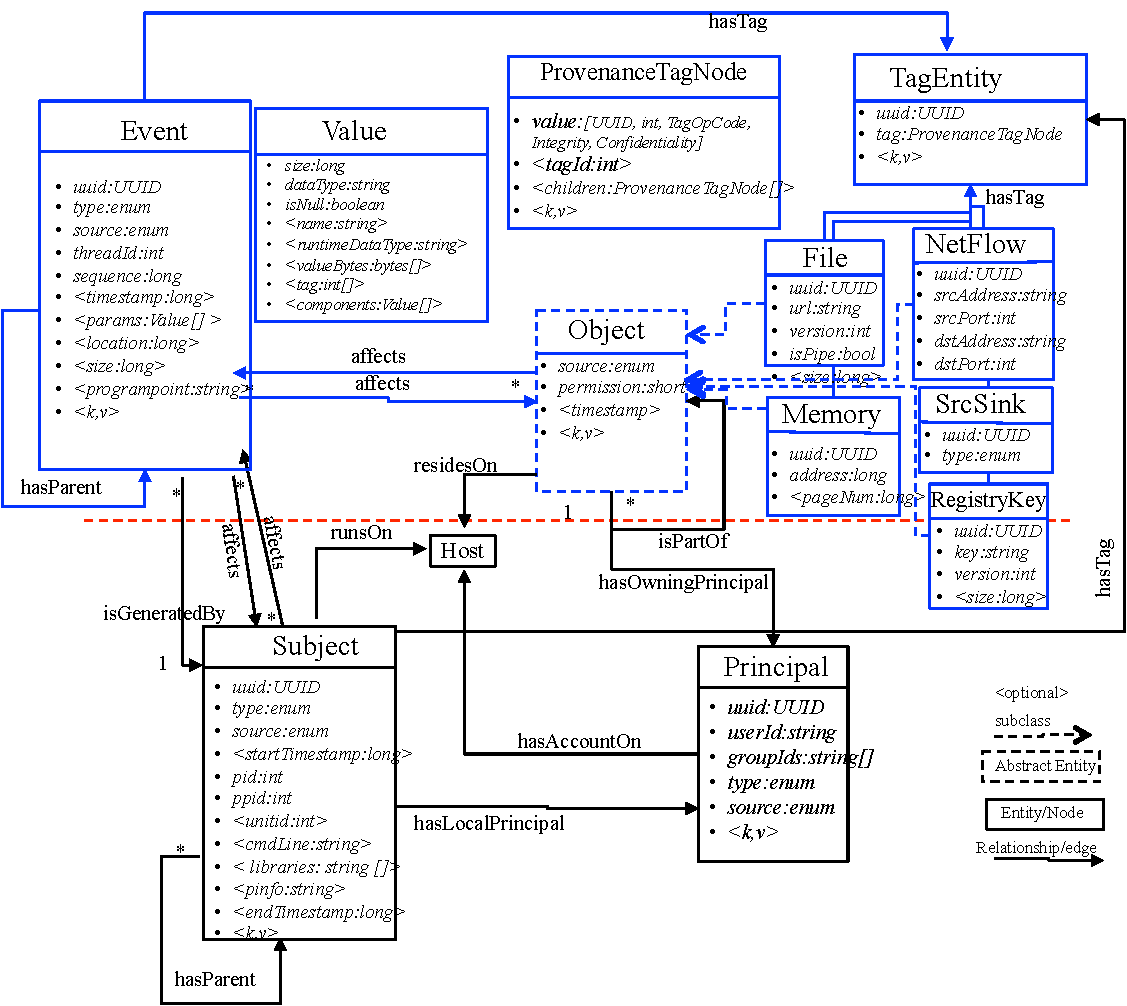
\includegraphics[width=0.9\textwidth]{graphmodel}
\caption{Conceptual common graph data model.}
\label{fig:erd}
\end{figure}

\section{Discussion}\label{sec:conceptual:credits}
As important as the model itself is the rationale for making some of the different design choices which we describe in this section.
As shown in Figure~\ref{fig:erd}, there are four core entities in the model: \textit{Events}, \textit{Subjects}, \textit{Objects}, and \textit{Tags}.
We added a \textit{source} attribute to the entities to identify the tracking system the data came from (e.g., OpenBSM, linux audit, TA1 tracker).

\subsection{Events and Subjects}\label{sec:conceptual:events}
Events represent actions executed on behalf of subjects. Events could include system calls, function calls at different layers, instruction executions, or even more abstract notions representing a ``blind'' execution such as black boxes that are not instrumented (more shortly). Events are the core entity in the model and they are the main abstraction for representing information flow between data objects, and subjects. 
Events are assumed to be atomic so there is no direct relationship between events (except for the meta-event described shortly). Instead, events are related to other events through the affected subjects and objects. 

Events can have different granularities but they are still atomic. For example, a function boundary may execute many atomic events within it, hence the function entry call would be captured as an event and so would the function exit call. The function boundary itself may be captured as a subject in this case if needed. If the function boundary is not instrumented however (black box), the function execution may still be captured as a ``blind'' event that relates the input and output subjects and objects (more on blindness shortly). 

Based on input from the CADETS team, we added the meta-event concept which allows grouping of a set of events under a single meta-event. This is represented using the event's \textit{hasParent} edge. The meta-event is clearly not atomic.

The event \textit{sequence} represents the logical order of the event relative to other events within the same execution thread. 
This could be the logical time, or if timestamps are accurate enough, \textit{sequence} might be inferred from timestamps but that is not guaranteed which is why we kept \textit{sequence}.
The event's \textit{location} and \textit{size} attributes (from ADAPT) are optional and they refer to the location and size of the data affecting the event (e.g., the read offset in the file and the number of bytes of data read for the read system call event).

Subjects represent execution contexts and include mainly threads and processes. They can be more granular and can represent other execution boundaries such as functions and blocks if needed. For example, a function within a thread within a process can be represented as three subjects where the function \textit{hasParent} thread, and the thread \textit{hasParent} process. Here the function subject is an execution boundary that is more granular than the thread (while we can represent this granularity, as of now it is unclear if and when this will be useful). 

An event \textit{isGeneratedBy} a subject. It may \textit{affect} other subjects such as when the output of a system call (event) forks a process (subject). A subject may \textit{affect} an event as well such as when the subject is the input to the event as is the case with the kill system call. 

An event \textit{affects} objects (more on objects in \S~\ref{sec:objects}). These may be the outputs of the event execution. Similarly, an object can \textit{affect} an event such as when the objects are input arguments to the event. Event parameters include input and output arguments to the event and are modeled as \textit{Value} attributes i.e., an event can have a array of Value records. Each Value record fully describes the data type of the value, its size, and its associated provenance taint/tag (more on tags later). Values, unlike system objects, are transient and are accordingly modeled as attributes to the Event instead of objects on their own. 

\paragraph{Events as first-class entities} In order to understand the rationale behind this, it is worth describing the alternative first. An alternative model (such as W3C PROV) treats events as binary edges between subjects and objects. These edges such as ``wasDerivedBy'' are annotated with event types and other metadata. While this is valid model, we found that treating events as edges creates unnecessary complexity in the model. This is especially true when events relate more than two objects and/or subjects. In this case, simulating this $n$-ary relationship using binary relationships complicates things. 
Instead, $n$-ary relationships may be natively supported in the common data model since events are vertices in the graph and they can be related to an arbitrary number of subjects and objects. 
It is important to note that it is straightforward to map this event-based model to a W3C PROV model if a TA2 should wish to do so: each event would be decomposed into a subset of the predefined PROV relations. This mapping may or may not be lossy depending on how accurately the PROV model would be able to capture the rich and complex semantics of system events. 
To avoid this mapping, we found it more natural and intuitive to use a more native event-based view.

\paragraph{Sensor blindness} An interesting discussion point raised by ADAPT was sensor blindness i.e., what happens when we don't have events (say with black boxes) but a TA1 technology is still able to capture the information flow into and out of the black box. We discussed two options here. In the first option, we can add edges directly between objects and between objects and subjects to represent this information flow. The other option that is more consistent with out event-based model is to create a special event type for ``blind'' events that still serves as the main entity for connecting the affected objects and subjects. We seemed to agree on the latter model. Hence, data can not flow directly between objects or subjects without going through an event. 

MARPLE and ADAPT identify a superset of events corresponding to system level calls. We need to agree on these event types. 

\subsection{Objects}\label{sec:objects}
Objects, in general, represent data sources and sinks which could include sockets, files, registry keys, memory and variables, and any data in general that can be an input and/or output to an event. This model expands the definition of objects to explicitly capture the flow of data inputs and outputs to and from events. 
We initially decided to treat event arguments as first class objects (instead of attributes of the event entity) where each object may have its own provenance again explicitly showing the flow from inputs to outputs. However we backed away from this later on as discussed shortly.
%Syscalls, functions, and instructions have inputs and outputs which could be objects or subjects. 

We identified some key object attributes. The object \textit{timestamp} is the creation time.  The file \textit{url} is its local or remote path/location. Files have version numbers. As files get updated, a new file object is created with a new version number. 

\paragraph{Transient data} 
One of the main discussion points was whether we should model arguments as Objects or whether we should explicitly distinguish transient data (e.g., arguments) from more persistent data (e.g., files). 
We agreed that it makes more sense to distinguish the two mainly because they have very different attributes (arguments don't have ownership and path attributes and have a value attribute). 
Initially, we decided to model a value as a first class entity, just like objects, that can have tags (discussed in \S \ref{sec:tags}) and \textit{affect} (and are affected by) events. 
We later decided (in version 0.7) to make values attributes of events instead of first class entities for the following reasons: values are one time constructs that only show up with the event and are not referenced afterwards during execution. TA-1 systems also do not track at the level  of a value. In addition, treating a value as a first class entity requires that we assign a unique ID to each value which does not scale since values can have byte granularity. As a result, we decided to make values attributes of the events.

\paragraph{Granularity and types} We discussed representing objects at various granularities. ADAPT modeled object containment using the \textit{isPartOf} relationship associated with the object/artifact. This allows us to represent a set of objects being part of a parent object, such as when writing buffers (objects with different tags) to a file (parent object). To explicitly differentiate between different types of objects, we also decided to subclass the abstract object into Files and Network Flows and Memory objects (and others we shall identify) instead of modeling those using a type attribute of the object entity. This is mainly to keep the model clean given the difference in attribute sets among the object types. 
We added the RegistryKey to model windows registry key store.
Finally, we also discussed whether we should model mobile phone sensors (GPS, camera, gyro, etc.) as a separate entity from Object, called Resource (as proposed in ADAPT). One observation here is that the sensing subsystem in Android for example might have enough differences to warrant this distinction. The counter argument is that Android uses linux underneath and one might be able to get away with an Object abstraction for all such data devices. For now, we decided to only distinguish File, RegistryKey, Netflow, Memory, and everything else uses the generic SrcSink object which is typed (e.g., sensors, camera, etc). 

\paragraph{Provenance} 
As discussed earlier, we explicitly model the relations between events and objects and subjects using the \textit{affects} relationship which is intended to identify the nature and semantics of the relation. 
The explicit relations between objects and events represents direct data flow (top part of Figure~\ref{fig:erd} in blue). 
%We discussed whether the \textit{affects} relationship should have a type attribute and it wasn't immediately clear what the types would be at this point, so we didn't include it. 
ADAPT defined a location attribute for the objects. This model made \textit{location} an attribute of the event instead since it is specific to the event (such as the location in a file where the read or write event happens).
The location may be the offset being read from a file or socket.
We similarly added \textit{size} as an optional attribute of the event. Edges between objects and events represent provenance directly in the graph. The complementary more granular approach uses tags, discussed next.

\subsection{Tags} \label{sec:tags}
The tag design was primarily fleshed out by the MARPLE team. The rationale for tags and their semantics is described next.

The primary motivation for tags is the ability to capture flows at a finer granularity and with increased precision. Specifically, tags can capture:
\begin{itemize}
\item {\em Increased precision:} Tags should be able to capture information flow  from a (strict) subset of inputs represented in a causality graph. For instance, a subject may read from 100 files, and then write one file. Rather than reporting that the output depends on these 100 inputs, a TA1 system can indicate that it depends only on 10th and 97th input files.
%
\item {\em Nature of dependence:} The behavior of the system can be understood in terms of a series of operations on inputs to produce outputs. Fine-grained tracking can identify the effect of these operations on data  flows. These effects can be described using {\em tag operations,} which can capture:
  \begin{itemize}
    \item common operations on data such as concatenation, mixing, compression, and so on.
    \item {\em declassification} and {\em endorsement,} the central operations used in information flow control literature
    \item strength of dependence, e.g., control dependence or implicit dependence
  \end{itemize}
%
\item {\em Flows involving internal (unreported) objects:} Especially for in-memory objects, not all updates and flows may be reported by a TA1 system. A TA1 system will internally keep track of these updates, and can then make the information available at the time when these objects contribute to an event argument.
%
\end{itemize}


Tags can be associated with entities (events, subjects, objects) using the edge \textit{hasTag} which connects say an Object with a TagEntity. 
The latter is simply a wrapper around the ProvenanceTagNode. The latter describes the actual tag expression. 
We describe the tag expression ProvenanceTagNode in more detail later in \S \ref{sec:provenancetag}.

Tags may also be directly associated with event parameters i.e., with Values, as attributes of the Value entity for fine grained taint tracking. 
Each Value has a tag which references a ProvenanceTagNode.

We identified three types of information captured by tags: (i) provenance (source dependence), (ii) confidentiality, and (iii) integrity, all of which can exist in parallel.
One can think of these tags forming three parallel planes each capturing a different aspect of data flow.
The integrity (respectively, confidentiality) may be used to specify the initial integrity (respectively, confidentiality) of data, 
or to {\em endorse} (respectively, {\em declassify}) its content after performing appropriate checking/sanitization.
%Multiple tags may be associated with any entity, e.g., an integrity
%and a confidentiality tag. Other examples are: (a) redefining a 
%complex tag expression as a new tag identifier, and (b) using a
%tag expression to capture full provenance, while also including 
%summary information in the form of an integrity or confidentiality label. 

In terms of the structure of tags, we defined the ProvenanceTagNode entity representing the full tag expression 
including provenance, confidentiality, and/or integrity.

\paragraph{Provenance information}
These define specific data sources (inputs). A tag identifier (an integer) is bound to a 
source and used by the tracking system to capture dependence on this source input.
This simple tree representation is expressive enough to capture all TA1 data but not too complicated.

\paragraph{Integrity information}
Integrity tags can have values {\em untrusted}, {\em benign}, or {\em invulnerable}.
The integrity tag {\em untrusted} indicates that the content is potentially malicious, 
while the tag {\em benign} indicates that it is from a source that is non-malicious\footnote{We need a
  suitable definition of {\em malice} --- for now, assume that non-malicious
  means that the content is not aimed at evading, circumventing, or violating a
  site's security policies.}. The tag {\em invulnerable} is applied only to
programs, and indicates that the program is trusted to be free of
vulnerabilities\footnote{The term {\em trusted} is used in the literature to
  refer to invulnerable programs, but we prefer the latter because (a) the term
  ``trusted'' is overused and often misunderstood, and (b) the term
  ``invulnerable'' conveys how strong the assumption is, driving home the point
  that it should be used very rarely.}$^{,}$\footnote{It would be clearer if
  integrity labels for programs are drawn from a different lattice than those
  for data files or processes. In particular, the terms ``invulnerable, benign''
  and ``untrusted'' apply to programs. For data files or processes, a two-valued
  domain with ``high'' and ``low'' would be more appropriate. However, this
  would require two different labels for executables, as they could be used as
  data or code. For this reason, we collapse the two domains, treating
  ``invulnerable'' and ``benign'' as being equivalent to ``high,'' and
  ``untrusted'' as being equivalent to ``low.''}.

\paragraph{Confidentiality tags}
Confidentiality tags can take values {\em secret}, {\em sensitive}, {\em private}, or {\em public}.
The label {\em secret} is meant for entities such as passwords. The label {\em
  sensitive} is used for all confidential data that needs to be protected, while
the {\em public} tag is reserved for information that can be freely shared with
the world. Non-public (but not confidential) data is designated {\em private.}

%A {\em tagOp} indicates how multiple information sources have
%been combined to produce an output. Its arguments can either be constants
%or other tag expressions. Some of the operators have very
%specific meaning, such as concatenation, while others aim to capture the
%degree of dependence (strong vs weak). 

\subsection{Extensibility Points} 
As everyone agrees, getting a complete and concise model right at the start is hard and we will need to define enough extensibility points to balance evolvability and conciseness. 

We are versioning the schema to track changes over time and adapt to them, as shown in version Table at the beginning of this document.

We also added extensibility points to the model like adding $<k,v>$ pairs to entities and relationships. We could also allow extending the types of entities. 

\subsection{Under considerations} 
The following additional aspects of the data model are still under consideration:
\begin{itemize}
\item We did not at this point separate the Resource from the Object (see \S~\ref{sec:objects})
\item Information flow between subjects and objects is captured through events in the current design. Whether we will allow direct flows between subjects and objects without going through events is still a point of discussion that we shall watch as we learn more about TA1s technologies especially since some TA1 trackers are focused solely on data flow traces, in which case forcing the data into an event based model might be overkill.
\item The model defined integrity and confidentiality tags. It is still unclear whether it is reasonable for TA2 to assume that a minimal initial set of confidentiality integrity tags can be provided by TA1s for key objects in the subjects in the system.
\item The need for subject tags and event tags is unclear at this point. Tags seem to be mostly relevant for values.
\end{itemize}

\section{Typed Schema Definition}\label{sec:syntax}

TA3 is developing a versioned and typed schema that codifies the above
conceptual model. The actual data model will necessarily evolve based
on the TA1-TA2 discussions expected in the coming months.  The schema
definition will evolve in parallel to match the latest version of the
data model.

The schema is specified using the Apache Avro Interface Description
Language (IDL) language. Avro IDL is a high-level language for
authoring Avro schemata. It provides a familiar feel for developers in
that it is similar to common programming languages like Java, C++, and
Python. Also, it is similar to IDLs in other serialization
frameworks such as Thrift and Protocol Buffers. Avro provides a tool
to convert the Avro IDL specification into an Avro schema in JSON
format, which is used by Avro serialization frameworks for automatic
serialization and deserialization of objects that conform to the schema.
Avro (and the TA3 APIs) additionally provide the tools for automatic 
syntax checking to verify the data conforms to the typed schema.

Both the schema and this documentation are kept in the same git repository 
and will evolve together. The latest development snapshot containing the evolving schema is
in a git repository shared with the rest of the TC team at the following URL 
\href{https://git.tc.bbn.com/bbn/ta3-serialization-schema/tree/master/avro}{https://git.tc.bbn.com/bbn/ta3-serialization-schema/tree/master/avro}. 
Look for the latest version $xx$ of the schema file {\em CDMxx.avdl}.


\section{Schema Detailed Description}
\subsection{Tags: ProvenanceTagNode and TagEntity}\label{sec:provenancetag}

We introduce the tag expression first, and then describe how we efficiently represent this granular expression using an in-memory data structure in Avro, the {\sf ProvenanceTagNode}.

The tag expression was originally proposed by the MARPLE team in their tags proposal,
and was slightly updated by BBN/MIT after a couple iterations working with the ClearScope data.
This tag design is suitable for a streaming model.
\footnote{The updates include mainly (1) removed the def and use, they seem unnecessary since a tagId is assigned the first time its used, (2) added a tagOp {\sf sequence} which is different than the union, (3) removed repeat op because I am separating the tag itself from the association of the tag with a value.}

The tag expression {\sf tagExpr} is a recursive structure with the following syntax:
\begin{Verbatim}[fontsize=\small]
 tagExpr := tagOp(tagExpr, tagExpr, ..) | tagId | UUID | integrityTag | confidentialityTag   
    tagOp := SEQUENCE | UNION | ENCODE | STRONG | MEDIUM | WEAK
    tagId  := int
    UUID := 256-bit ID //universally unique identifier of an entity 
    integrityTag := UNTRUSTED | BENIGN | INVULNERABLE
    confidentialityTag := SECRET | SENSITIVE | PRIVATE | PUBLIC
\end{Verbatim}

A {\sf tagId} is an integer that uniquely identifies a tag expression. This could be as simple as referencing a source Object UUID (e.g., when the tagExpr := UUID) or could reference a more complex nested tag expression. A tagId is defined only once and used later in other tag expressions (the assignment of a tagId to an expression in not shown in the syntax above, but will be described later).
The tagId is not to be confused with {\sf UUID} which is a universally unique id for identifying arbitrary entities in the model (such as objects, subjects, and events). UUIDs are defined and emitted with their respective entities, and only referenced as part of the tag expressions.

A {\sf tagOp} is a tag operator that describes how different data inputs are combined to produce an output.
We identified a small subset of tag operators above with the following semantics: 
\begin{itemize}
\item {\sf SEQUENCE}: SEQUENCE(y, x) means that the output was derived from x then y in that sequential order. This is different than the UNION opcode which is flat. We added SEQUENCE mainly to represent the {\em prev-Tag} semantics used by ClearScope. Specifically, ClearScope tracks propagation of tags across process boundaries. For example, data with tag x can be written to a file by a process A, then read from the file into some variable y by process B. The variable y will have a new tag and a {\em prev-tag}=x. So the {\em prev-tag}s can be chained to track provenance across object and process boundaries and there is a clear sequence.
\item {\sf UNION}: this is the most common operator denoting that inputs are somehow merged to create the output. 
\item {\sf \{STRONG | MEDIUM | WEAK\}}: are more vague and designate a {\em degree of dependence} rather than a very specific operator.
\end{itemize}

A {\sf ProvenanceTagNode} codifies a tag expression efficiently on the wire (in our case, using Avro). ProvenanceTagNode is a tree where each Node in the tree has a value and an ordered list of children Nodes to capture the recursive structure of {\sf tagExpr}:
\begin{Verbatim}[fontsize=\small]
    record ProvenanceTagNode {
        union {int, UUID, TagOpCode, IntegrityTag, ConfidentialityTag} value;
        array<ProvenanceTagNode> children = null; //optional
        int tagId; //optional
        map<string> properties; //optional
    }
\end{Verbatim}
The ProvenanceTagNode.value is a union which means it can be either an int (tagId), a UUID, a TagOpCode, or an integrity or confidentiality tag. 
The ProvenanceTagNode.tagId assigns an int tag identifier to this ProvenanceTagNode instance. Think of a table indexed by tagId where each unique tagId maps to a ProvenanceTagNode instance (the tag expression). Here ProvenanceTagNode.tagId is the index column for the ProvenanceTagNode instance. Once the tagId is assigned, it may be referenced in future tag expressions within ProvenanceTagNode.value.

Take a simple example: say an instrumentation system assigns a tagId=1 to all bytes read from a netflow object whose UUID=uuid1. Using CDM, this means there is a netflow object with UUID=uuid1 that was emitted before the bytes are read. Then a ProvenanceTagNode is emitted as follows:
\begin{Verbatim}[fontsize=\small]
    ProvenanceTagNode {
        value=uuid:uuid1,
        tagId=int:1
    }
\end{Verbatim}
This means that tagId 1 refers to the entity (in this case source object) with uuid1. Now this tagId can be assigned to the data bytes or can be used in other composite tag expressions (we will describe how tags are assigned to data and entities shortly).

Now say data from the netflow object uuid1 is combined with data from another source object with UUID=uuid2 to produce an output. The provenance of the output data may be described using the simple expression, 
\begin{Verbatim}[fontsize=\small]
UNION(UUID:uuid1, UUID:uuid2)
\end{Verbatim}
which is equivalent to the expression
\begin{Verbatim}[fontsize=\small]
UNION(int:1, UUID:uuid2)
\end{Verbatim}
because we previously assigned tagId int:1 to the source object with UUID:uuid1. This new tag expression may be represented using ProvenanceTagNode as follows:
\begin{Verbatim}[fontsize=\small]
    ProvenanceTagNode { // corresponding to UNION(int:1, UUID:uuid2)
        value=TagOpCode.UNION,
        tagId=int:5,
        children = [
             ProvenanceTagNode {
               value=int:1
            },
             ProvenanceTagNode {
               value=uuid:uuid2
           },
        ],
    }
\end{Verbatim}
where we have a root Node that represents the full expression with two child nodes, one corresponding to each of the constituent tag expressions within the UNION operator. 
The tag expression gets assigned a tagId int:5.
There are several equivalent representations of the same expression just as we showed earlier. For example, we could have emitted a Node for uuid2 separately and just referenced
it in the new tag expression as follows:
\begin{Verbatim}[fontsize=\small]
    ProvenanceTagNode {
       value=uuid:uuid2,
       tagId=int:2
    }
    
    ProvenanceTagNode { // corresponding to UNION(int:1, int:2)
        value=TagOpCode.UNION,
        tagId=int:5,
        children = [
             ProvenanceTagNode {
               value=int:1
            },
             ProvenanceTagNode {
               value=int:2,
            }
        ]
    }
\end{Verbatim}
Note that when parsing ProvenanceTagNode record, all the fields are typed so by checking the type of the value, one can know whether this is an int (reference to another tag expression) or a UUID (reference to an entity).

Now that we explained how one can create a granular tag expression, we describe how tags may be assigned to data and entities in the model. 
We can assign tags to transient data, specifically the event's parameters which are Values, or we can assign tags to persistent entities (events, subjects, objects) directly.

{\em Value tags:} Events such as system calls typically involve input and output parameters which are modeled in CDM as {\sf Value}s. Event.parameters is an array of Values, where each value may have its own tag. Here we describe the value tags only, and we defer the detailed explanation of Value record itself to \S \ref{sec:values}. Value.tag is an array of integers that uses the run-length encoding to express the tags associated with the different elements in the value-- the value can be an array. In other words, we separate the association of the tag with the Value from the tag expression itself. 
The format of the run-length encoded tag array associated with the value is:
\begin{Verbatim}[fontsize=\small]
{<numElements:int>, <tagId:int>}*
\end{Verbatim}
For example, assume value is an array int[16]. To assign a tag 0 (unknown) to elements 0-3, tag 1 to elements 4-7, and tag 2 to elements 8-15 of
the array, this would be represented using the following tag array:
\begin{Verbatim}[fontsize=\small]
{4, 0, 4, 1, 8, 2}
\end{Verbatim}
meaning the first 4 elements have tag 0, next 4 have tag 1, next 8 have tag 2.
Note that 4 elements of the int array correspond to 16 bytes.
Also note that the tagIds 1 and 2 had to be defined and emitted earlier using ProvenanceTagNode before they are assigned to a value.
We provide more examples from ClearScope, and FAROS shortly.

{\em Entity tags:} Tags may be associated with entities such as events, subjects, and objects. An entity can have multiple tags, and more importantly entity tags may be added incrementally over time. For example, the THEIA system creates and emits entities at runtime, and then later at some future time attaches more tags to the entities (e.g., after they do the offline analysis). Our design for assigning these multiple incremental tags to the entities is using an edge {\sf hasTag} from the entity (e.g. File) to a {\sf TagEntity} entity. The latter simply wraps the ProvenanceTagNode with a uuid so that we can create an edge to it (recall our simple edge design connects two entities using their UUIDs, and ProvenanceTagNode is not an entity). 

Now that we described how tag expressions can be modeled efficiently on-the-wire, lets work through some examples of tag expressions. Note that in the examples that follow, I edited the json CDM output for brevity.\\

\noindent \underline{MIT/ClearScope Examples:}

Consider the following raw trace from the ClearScope instrumentation (before it is translated to CDM):
\begin{Verbatim}[fontsize=\small]
define src-type 2 : LOCATION
define prov 1001 : src-type=2, app-ppt=1, prev-tag=0
...
define src-type 10 : ENVIRONMENT OFFSET
define prov 1003 : src-type=10, app-ppt=9, prev-tag=0
define prov-set 1004 : 1001, 1003
...
define sink-type 14 : FILE /tmp/photo.png
define prov 1005 : sink-type=14, app-ppt=12, prev-tag=1004
sink program=1000, app-ppt=12, sys-call=13, sink-type=14, tid=1, time=2016-04-05T15:26:03.067-04
  sink float 
    v: 72.120600
    md: 1005
\end{Verbatim}
The trace is straightforward to understand: an int tagId {\sf 1001} is assigned to the {\sf LOCATION} source (at program point app-ppt=1). Using our tag expression syntax, and given the {\sf LOCATION} source object has a UUID=2, this corresponds to first creating and emitting the following tag expression:
\begin{Verbatim}[fontsize=\small]
    ProvenanceTagNode {
       value=uuid:2,
       tagId=int:1001,
       properties={
           "app-ppt": <ppt info>
       }
    }    
\end{Verbatim}
Similarly for tag expression 1003 assigned to the source object SOURCE\_ENV\_VARIABLE,
\begin{Verbatim}[fontsize=\small]
    ProvenanceTagNode {
       value=uuid:10,
       tagId=int:1003,
       properties={
           "app-ppt": <ppt info>
       }
    }    
\end{Verbatim}
Then a new tag expression is defined for the representing the provenance of combining the two sources above using a UNION operator,
\begin{Verbatim}[fontsize=\small]
    ProvenanceTagNode { // corresponding to UNION(int:1001, int:1003)
        value=TagOpCode.UNION,
        tagId=int:1004,
        children = [
             ProvenanceTagNode {
               value=int:1001
            },
             ProvenanceTagNode {
               value=int:1002
            }
        ]
    }
\end{Verbatim}
A new tag expression with tagId 1005 is then defined for writing data to a sink FileObject object and using the prev-tag defined earlier to denote where the data came from before it was written to the sink file. To represent the prev-tag information, we use the TagOpCode.SEQUENCE operator as follows,
\begin{Verbatim}[fontsize=\small]
    ProvenanceTagNode { // corresponding to SEQUENCE(uuid:14, int:1004)
        value=TagOpCode.SEQUENCE,
        tagId=int:1005,
        children = [
             ProvenanceTagNode {
               value=uuid:14, // the FILE object 
               properties={
                   "app-ppt": <ppt info>
                }
             },
             ProvenanceTagNode {
               value=int:1004
            }
        ]
    }
\end{Verbatim}
Finally, the tag expression is assigned to the output value within the event corresponding to write sys-call as follows,
\begin{Verbatim}[fontsize=\small]
  Event {
      uuid : 74DE390,
      sequence : 5,
      type : EVENT_WRITE,
      ...
      parameters : [ { //array of Value records, a single primitive Vlaue in this case
          size : -1,
          type : VALUE_TYPE_OUT,
          valueDataType : VALUE_DATA_TYPE_FLOAT,
          isNull : false,
          runtimeDataType : null,
          valueBytes : {
            bytes : 42903DBF
          },
          tag : {
            array : [ -1, 1005 ]
          }
        } ],
   }
\end{Verbatim}
The tag array [ -1, 1005 ] associated with the event parameter means that the parameter which is a primitive (of size -1) has a tag expression with tagId 1005, which was defined/emitted earlier. Using our run-length encoding, starting with -1 (=size) in the array means all the Value elements have the specified tag.\\


\noindent \underline{UNM/FAROS Examples:}

The current representation used by FAROS (which is still evolving) is very similar to the above. Consider the following sample raw output from FAROS,
\begin{Verbatim}[fontsize=\small]
NewProvenanceTagNode 1 2b2946e1fd99d6df...
NewEvent e92dcbfb141c40deb458... 0 EVENT_UNKNOWN 1236 1462744526664000 389 NtWaitForMultipleObjects 6
|--NewValue 4 VALUE_TYPE_IN VALUE_DATA_TYPE_BYTE 25000000 [4,1] 
|--NewValue 4 VALUE_TYPE_IN VALUE_DATA_TYPE_BYTE 30FF1200 [4,1] 
|--NewValue 4 VALUE_TYPE_IN VALUE_DATA_TYPE_BYTE 01000000 [4,1] 
|--NewValue 4 VALUE_TYPE_IN VALUE_DATA_TYPE_BYTE 01000000 [4,1] 
|--NewValue 4 VALUE_TYPE_IN VALUE_DATA_TYPE_BYTE 00000000 [4,1] 
|--NewValue 1 VALUE_TYPE_OUT long 36
\end{Verbatim}
A tag expression with tagId 1 is defined, and then assigned (using the run-length encoding) to 5 parameters of type byte [4] read by an Event. 
The tag expression and event is translated to CDM as follows,
\begin{Verbatim}[fontsize=\small]
ProvenanceTagNode {
      value=uuid:2B2946E1FD99D6DF...,
      tagId=int:1
}

Event {
      uuid : E92DCBFB141C40DEB458...,
      sequence : 0,
      type : EVENT_UNKNOWN,
	...
      name="NtWaitForMultipleObjects",
      parameters= [ {
          size : 4,
          type : VALUE_TYPE_IN,
          valueDataType : VALUE_DATA_TYPE_BYTE,
          isNull : false,
          runtimeDataType : null,
          valueBytes : 25000000,
          tag : [ 4, 1 ]
        }, {
          size : 4,
          type : VALUE_TYPE_IN,
          valueDataType : VALUE_DATA_TYPE_BYTE,
          isNull : false,
          runtimeDataType : null,
          valueBytes : 30FF1200,
          tag :  [ 4, 1 ]
        }, 
        ... // another 2 input params same as above, and an output param
        } ]
  ...
}
\end{Verbatim}
Note that FAROS team is in the process of propagating provenance across merges (UNION operator) and updating the event types and making other changes.

\subsection{Value}\label{sec:values}
{\sf Value}s used as event parameters can model different data types including primitive data types (byte, bool, char, short, int, long, float, double), complex data types like objects which comprise primitive or other complex types, and arrays of primitive and complex types. The Value design is well document in the CDM avdl schema file (CDM12.avdl as of this writing). Here we highlight the aspects that might not be immediately clear using some examples.

The Value.size is used to distinguish between arrays (size $\ge$ 0), and non-arrays (size < 0) i.e., whenever size is $\ge$ 0, the Value should be interpreted as an array of type Value.valueDataType. The latter can be primitive or complex data type as described in the schema. Complex values generally comprise other values, hence they use the Value.components=Value[] as a recursive structure.

The Value.isNull flag indicates whether the value is null and is needed to distinguish null values from those not null but with size $\le$ 0.

A string is always modeled as an array of chars using UTF32\_BE (32 bits per character in big endian). Hence, a non-null string value will have size $\ge$ 0 and Value.valueDataType=VALUE\_DATA\_TYPE\_CHAR. This is to simplify things since each character in a string may have its own tag.

We additionally have the Value.runtimeDataType to indicate the actual runtime data type of the Value which could be anything. For example, a class of type MyClass that comprises of a string and an int might look like the following,
\begin{Verbatim}[fontsize=\small]
   Value {
          size : -1,
          type : VALUE_TYPE_IN,
          valueDataType : VALUE_DATA_TYPE_COMPLEX,
          isNull : false,
          runtimeDataType : "MyClass",
          valueBytes : null,
          tag :  null,
          components : [ 
            { // first the string, say "0123"
                  size : 4,
                  type : VALUE_TYPE_IN,
                  valueDataType : VALUE_DATA_TYPE_CHAR,
                  isNull : false,
                  runtimeDataType : String,
                  valueBytes : 00000030000000310000003200000033, //UTF32_BE
                  tag :  [ 4, 1 ]
            },
            { // and an int, say 0
                  size : -1,
                  type : VALUE_TYPE_IN,
                  valueDataType : VALUE_DATA_TYPE_INT,
                  isNull : false,
                  runtimeDataType : null,
                  valueBytes : 00000030,
                  tag :  [ -1, 2 ]
            }]
  }
\end{Verbatim} 
Notice how we used runtimeDataType=String if we want to highlight that something is a string instead of a char[].

%\begin{Verbatim}[fontsize=\small]
%\end{Verbatim}


\end{document}
